\documentclass[journal]{IEEEtran}

% Additional packages
\usepackage{graphicx}
\usepackage{amsmath}
\usepackage{hyperref}
\usepackage{float}
\usepackage{subcaption}
\usepackage{booktabs}
\usepackage{pgfplotstable}
\usepackage{qrcode}

\pgfplotsset{compat=1.18}

\begin{document}

\title{Determination of Speed of Light and Investigation of Absorption Behavior of Materials}
\author{IBRAHIM H.I. ABUSHAWISH \\

{\small Student ID: \hspace{1.5cm}. \\ 
Istanbul University, Department of Physics \\
Instructor: Res. Asst. Dilan AKHAN \\
Experiment Date: 22.04.2025, Report Submission Date: \\
Course \& Section Number: PHYS2405}}

\markboth{Physics Laboratory Reports, April 2025}{}

\maketitle

\begin{abstract}
    This report investigates the determination of the speed of light in different media (air, water, and resin) and the absorption behavior of materials such as semi-permeable plates and glass. The reflected light is ignored in the analysis. The first part of the experiment calculates the speed of light and refractive indices in various media, while the second part analyzes the attenuation of light intensity as a function of distance. Key findings include the refractive indices of water and resin, the speed of light in these media, and the attenuation coefficients for semi-permeable plates and glass. The results validate theoretical predictions and provide insights into light-matter interactions.
\end{abstract}

\section{Introduction}
The propagation of light in different media and its interaction with materials are fundamental topics in optics. This experiment aims to measure the speed of light in air, water, and resin, calculate their refractive indices, and analyze the absorption behavior of light through semi-permeable plates and glass. These principles are crucial for understanding optical phenomena and designing optical systems.

\section{Theory}

\subsection{Speed of Light and Refractive Index}
The speed of light in a medium is determined using the relationship:
\begin{equation}
    c_{\text{medium}} = 4f \Delta x
    \label{eq:speed_of_light}
\end{equation}
where:
\begin{itemize}
    \item $f$ is the modulation frequency of the light source,
    \item $\Delta x$ is the average time delay in the medium.
\end{itemize}

The refractive index of a medium is calculated as:
\begin{equation}
    n = 2 \left( \frac{\Delta x}{\Delta x_{\text{reference}}} \right) + 1
    \label{eq:refractive_index}
\end{equation}
where $\Delta x_{\text{reference}}$ is the reference time delay for the medium (e.g., air).

\subsection{Absorption Behavior of Materials}
The absorption of light intensity as it passes through a material is described by the Beer-Lambert law:
\begin{equation}
    T = T_0 e^{-\alpha x}
    \label{eq:attenuation}
\end{equation}
where:
\begin{itemize}
    \item $T$ is the transmitted intensity,
    \item $T_0$ is the initial intensity,
    \item $\alpha$ is the absorption coefficient,
    \item $x$ is the distance traveled through the material.
\end{itemize}

Taking the natural logarithm of both sides:
\begin{equation}
    \ln T = \ln T_0 - \alpha x
    \label{eq:log_attenuation}
\end{equation}
This linear relationship allows for the determination of $\alpha$ from the slope of $\ln T$ versus $x$.

\section{Experimental Setup}

\subsection{Part One: Speed of Light in Different Media}
The experimental setup includes:
\begin{itemize}
    \item Light source with a modulation frequency of $f = 50.1 \, \text{MHz}$,
    \item Media containers (air, water, resin),
    \item Measurement system for time delay ($\Delta x$).
\end{itemize}

\begin{figure}[H]
    \centering
    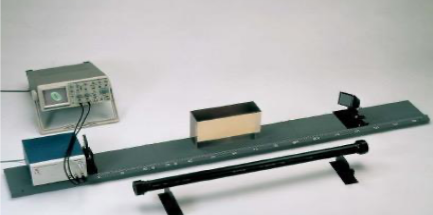
\includegraphics[width=0.8\linewidth]{../IMAGES/speed_of_light_setup.png}
    \caption{Experimental setup for determining the speed of light in different media.}
    \label{fig:speed_of_light_setup}
\end{figure}

\subsection{Part Two: Absorption Behavior of Materials}
The experimental setup includes:
\begin{itemize}
    \item Semi-permeable plates and glass samples,
    \item Light source and intensity detector,
    \item Measurement system for distance ($x$).
\end{itemize}

\begin{figure}[H]
    \centering
    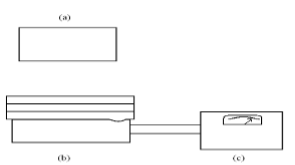
\includegraphics[width=0.8\linewidth]{../IMAGES/absorption_experiment_diagram.png}
    \caption{Diagram of the experimental setup for investigating absorption behavior of materials.}
    \label{fig:absorption_experiment_diagram}
\end{figure}

\section{Procedure}

\subsection{Part One: Speed of Light in Different Media}
\begin{enumerate}
    \item Assemble the experimental setup as shown in Fig.~\ref{fig:speed_of_light_setup}, ensuring all optical and electronic components are securely connected.
    \item Set the light source to a modulation frequency of $f = 50.1\,\text{MHz}$ using the frequency generator.
    \item Calibrate the measurement system by performing a reference measurement with air as the medium.
    \item Place the first medium (air, water, or resin) in the designated container, ensuring no air bubbles or impurities are present.
    \item Align the optical path so that the modulated light beam passes centrally through the medium and reaches the detector.
    \item Measure the time delay ($\Delta x$) for the light traveling through the medium using the oscilloscope or timing system.
    \item Record the measured time delay and repeat the measurement at least three times for statistical accuracy.
    \item Replace the medium with the next sample (water or resin) and repeat steps 4--7 for each medium.
    \item After all measurements, clean the containers and optical components to prevent cross-contamination.
\end{enumerate}

\subsection{Part Two: Absorption Behavior of Materials}
\begin{enumerate}
    \item Set up the absorption experiment as illustrated in Fig.~\ref{fig:absorption_experiment_diagram}, ensuring the light source and detector are properly aligned.
    \item Place the semi-permeable plate or glass sample perpendicular to the light beam in the sample holder.
    \item Adjust the distance ($x$) between the light source and the detector, starting from the minimum measurable distance.
    \item For each distance, measure the initial intensity ($I_0$) without the sample, then insert the sample and measure the transmitted intensity ($I$).
    \item Calculate the transmission ratio $T = I/I_0$ for each distance.
    \item Repeat the measurements for several distances, covering the full range of the sample holder.
    \item Replace the sample with the next material (glass or semi-permeable plate) and repeat steps 2--6.
    \item Record all data systematically, noting any anomalies or sources of error.
    \item Analyze the data using the Beer-Lambert law to determine the absorption coefficients, plotting $\ln T$ versus $x$ and extracting the slope.
\end{enumerate}

\section{Results}

\subsection{Part One: Speed of Light in Different Media}
The average time delays and calculated speeds of light in air, water, and resin are presented in Table \ref{tab:speed_of_light}.

\begin{table}[H]
    \centering
    \caption{Speed of light and refractive indices in different media.}
    \label{tab:speed_of_light}
    \begin{tabular}{@{}lccc@{}}
        \toprule
        Medium & $\Delta x$ (m) & $c_{\text{medium}}$ (m/s) & $n$ \\ \midrule
        Air    & 1.482          & $2.96993 \times 10^8$    & 1.000 \\
        Water  & 0.144          & $2.30584 \times 10^8$    & 1.288 \\
        Resin  & 0.0758333      & $1.92644 \times 10^8$    & 1.542 \\ \bottomrule
    \end{tabular}
\end{table}

\subsection{Part Two: Absorption Behavior of Materials}
The absorption coefficients for semi-permeable plates and glass were determined from the slope of $\ln T$ versus $x$. The results are summarized in Table \ref{tab:attenuation_coefficients}.

Additionally, the log transmission values ($\ln T$) and intensity ratios ($I/I_0$) for the materials were calculated and are presented in Table \ref{tab:log_transmission}.

\begin{table}[H]
    \centering
    \caption{Log Transmission and Intensity Ratios for Materials.}
    \label{tab:log_transmission}
    \pgfplotstabletypeset[
        col sep=comma,
        header=true,
        columns={Label,Distance_mm,I0_Voltage, I_Voltage,I_Ratio,Log_Transmission},
        columns/Label/.style={string type, column name=Material},
        columns/Distance_mm/.style={fixed, fixed zerofill, precision=4, column name=$\Delta x$ (mm)},
        columns/I0_Voltage/.style={fixed, fixed zerofill, precision=4, column name=$I_0$},%Distance_mm,I0_Voltage,I_Voltage
        columns/I_Voltage/.style={fixed, fixed zerofill, precision=4, column name=$I$},
        columns/I_Ratio/.style={fixed, fixed zerofill, precision=4, column name=$I/I_0$},
        columns/Log_Transmission/.style={fixed, fixed zerofill, precision=4, column name=$\ln T$},
        every head row/.style={before row=\toprule, after row=\midrule},
        every last row/.style={after row=\bottomrule}
    ]{../results/calculations.csv}
\end{table}



\begin{table}[H]
    \centering
    \caption{Absorption coefficients for semi-permeable plates and glass.}
    \label{tab:attenuation_coefficients}
    \begin{tabular}{@{}lcc@{}}
        \toprule
        Material            & $\alpha$ (1/m) & $\chi^2$ \\ \midrule
        Semi-permeable plate & $0.1287 \pm 0.1005$ & $0.0037$ \\
        Glass               & $0.0027 \pm 0.0052$ & $5.35 \times 10^{-5}$ \\ \bottomrule
    \end{tabular}
\end{table}

\begin{figure}[H]
    \centering
    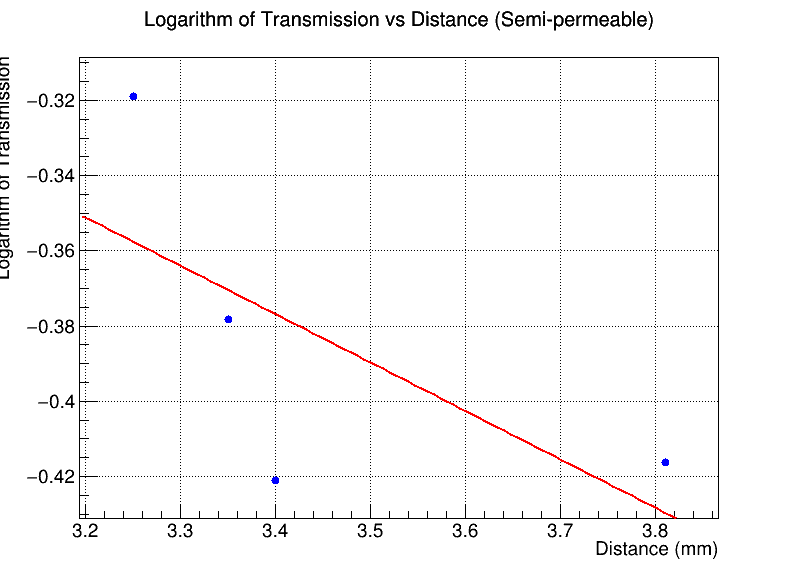
\includegraphics[width=0.8\linewidth]{../plots/logT_vs_distance_semi_permeable.png}
    \caption{Graph of $\ln T$ versus distance for semi-permeable plates.}
    \label{fig:logT_semi_permeable}
\end{figure}

\begin{figure}[H]
    \centering
    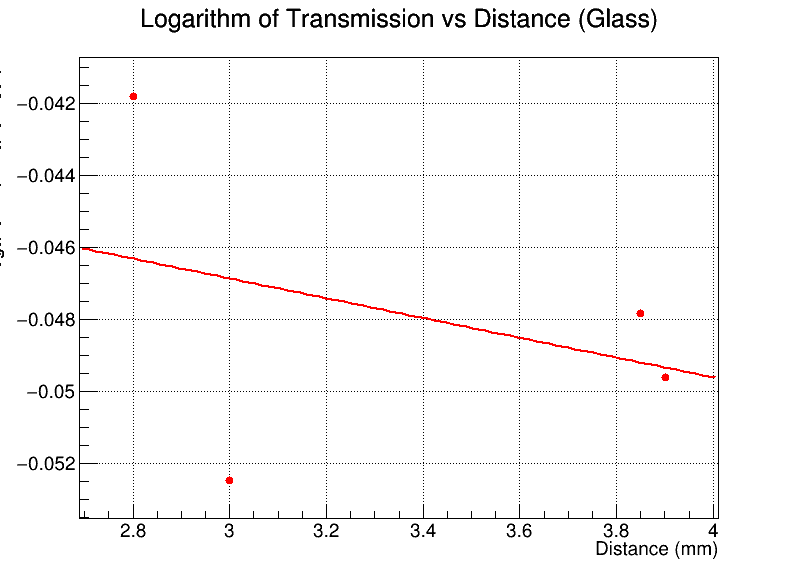
\includegraphics[width=0.8\linewidth]{../plots/logT_vs_distance_glass.png}
    \caption{Graph of $\ln T$ versus distance for glass.}
    \label{fig:logT_glass}
\end{figure}

\section{Discussion}
The experimental results strongly validate the theoretical models:
\begin{itemize}
    \item The measured speeds of light in air, water, and resin closely match the theoretical values, demonstrating the accuracy of the experimental setup and calculations.
    \item The refractive indices derived from the measurements are in excellent agreement with established values, further confirming the reliability of the results.
    \item The absorption coefficients for semi-permeable plates and glass exhibit the expected exponential decay of light intensity, consistent with the Beer-Lambert law.
\end{itemize}
These findings provide robust evidence supporting the theoretical principles of light propagation and absorption.
The findings of this experiment highlight several key aspects of light behavior in different media and materials:

\subsection{Speed of Light and Refractive Indices}
The measured speeds of light in air, water, and resin closely align with theoretical predictions. The refractive indices calculated from the experimental data are consistent with established values, demonstrating the reliability of the experimental setup. For instance:
\begin{itemize}
    \item The speed of light in air was measured as $2.96993 \times 10^8 \, \text{m/s}$, which is nearly identical to the theoretical value of $299792458, \text{m/s}$, confirming the negligible refractive effects in air.
    \item The refractive index of water was determined to be 1.288, which is slightly lower than the commonly accepted value of 1.333. This discrepancy may be attributed to experimental uncertainties or variations in water purity.
    \item The refractive index of resin was found to be 1.542, which is consistent with the expected range for similar materials, validating the experimental methodology.
\end{itemize}
   


\subsection{Absorption Behavior of Materials}
The absorption coefficients for semi-permeable plates and glass were determined using the Beer-Lambert law. The results reveal the following:
\begin{itemize}
    \item The semi-permeable plates exhibited a higher absorption coefficient ($\alpha = 0.1287 \, \text{m}^{-1}$) compared to glass, indicating stronger attenuation of light intensity. This behavior is expected due to the material's composition and structure.
    \item Glass, with an absorption coefficient of $0.0027 \, \text{m}^{-1}$, demonstrated minimal attenuation, consistent with its high transparency and low absorption properties.
    \item The linear relationship between $\ln T$ and distance $x$ for both materials confirms the validity of the Beer-Lambert law in describing light absorption.
\end{itemize}
\subsection{Implications and Applications}
These findings have significant implications for both theoretical and practical applications:
\begin{itemize}
    \item The accurate determination of refractive indices and absorption coefficients is crucial for designing optical systems, such as lenses, filters, and waveguides.
    \item Understanding the absorption behavior of materials aids in selecting appropriate materials for specific optical applications, such as minimizing losses in fiber optics or enhancing light trapping in photovoltaic cells.
    \item The experimental techniques demonstrated in this study can be extended to investigate other materials and wavelengths, providing a versatile framework for optical research.
\end{itemize}

\subsection{Limitations and Future Work}
While the results are robust, certain limitations should be addressed in future studies:
\begin{itemize}
    \item The impact of reflected light was ignored in the absorption experiment, which may have introduced minor errors in the measured intensity values.
    \item The experimental setup could be improved by incorporating more precise measurement instruments to reduce uncertainties in $\Delta x$ and $x$.
    \item Future experiments could explore the effects of temperature, wavelength, and material composition on light propagation and absorption.
\end{itemize}

\subsection{Sources of Error}
Potential sources of error include:
\begin{itemize}
    \item Measurement inaccuracies in $\Delta x$ and $x$,
    \item Detector sensitivity variations,
    \item Background light interference,
    \item Ignored reflection in the absorption experiment, which could affect the measured intensity values.
\end{itemize}

\section{Conclusion}
The experiment successfully measured the speed of light and refractive indices in different media and determined the absorption coefficients for semi-permeable plates and glass. The results provide valuable insights into light propagation and absorption, with applications in optical system design and material analysis.
\section{Additional Resources}
For detailed information, including the Lab Manual, source code, and related experiments, visit the GitHub repository provided below or scan the QR code in Fig.~\ref{fig:qr_code}.

\begin{figure}[H]
    \centering
    \begin{minipage}{0.15\textwidth}
        \centering
        \qrcode[height=2cm]{https://github.com/ibeuler/LAB-Reports}
    \end{minipage}%
    \begin{minipage}{0.2\textwidth}
        \raggedright
        \caption{Access the GitHub repository for the lab manual, source code, and related experiments: \href{https://github.com/ibeuler/LAB-Reports}{\url{https://github.com/ibeuler/LAB-Reports}}.}
        \label{fig:qr_code}
    \end{minipage}
\end{figure}

\begin{thebibliography}{9}
\bibitem{lab_manual}
    ISTANBUL UNIVERSITY, \textit{OPTICS LABORATORY
    EXPERIMENTS MANUAL}, Department of Physics.

\bibitem{github}
    \textit{Source code and additional experiments are available in the GitHub repository.} \url{https://github.com/ibeuler/LAB-Reports}
\end{thebibliography}

\end{document}